\documentclass{beamer}

% \usepackage{mdframed}
\usepackage[utf8]{inputenc}
\usepackage{default}



\begin{document}

	\title[Crisis]{Secure Two Party Computation}
	\subtitle{Preliminary presentation}
	\author[Author]{Nick Tutte\\[1ex]{\tiny Prof. Nigel Smart}}
	\date[Feb 2015]
	{February, 2015}
	\subject{Computer Science}
	\frame{\titlepage}
	\setbeamertemplate{caption}[numbered]


	\begin{frame}
		\frametitle{Presentation overview}
		\begin{itemize}
			\item My project focuses on Secure Multiparty Computation, in particular the two party case using Yao Garbled Circuits.
			\item I shall be implementing the as yet unimplemented protocol laid out by Lindell in ``Fast Cut-and-Choose based Protocol for Malicious and Covert Adversaries.''

			\item By the end of this presentation you should know,
			\begin{itemize}
				\item What is Secure Multiparty Computation?
				\item What can it be used for?
				\item What ``Secure'' means in this context.
				\item A grounding in Yao Garbled Circuits.
				\item How much progress I've made so far.
			\end{itemize}
		\end{itemize}

	\end{frame}


	\begin{frame}
		\frametitle{What is Secure Multiparty Computation?}
		
		\begin{itemize}
			\item In the problem of Secure Multiparty Computation we have a set of parties, each of whom has a secret input.
			\item The parties wish to co-operate to compute a function upon their collective inputs without revealing said inputs to one another.
			\item Some example applications are,
			\begin{itemize}
				\item The Millionaires problem.
				\item Distributed secrets.
				\item Sugar Beets.
				\item Database query.
			\end{itemize}
		\end{itemize}
	\end{frame}



	\begin{frame}
		\frametitle{Desired security properties}

		Before we go any further we need to define what properties we want an SMC protocol to fulfill before we consider it Secure.
		
		\begin{itemize}
			\item \textbf{Privacy}, the only knowledge parties gain from participating is the output.
			\item \textbf{Correctness}, the output is indeed that of the intended function.
			\item \textbf{Independence of inputs}, no party can choose it's inputs as the function of other parties inputs.
			\item \textbf{Fairness}, corrupt parties receive their outputs if and only if the honest parties also receive their outputs.
		\end{itemize}

		% Privacy - Note this is very dependent on the function. For example if the function is simple addition then clearly an adversary can calculate the other parties input as the output minus its own input. But the only information they gain is their intended output.
		% Correctness - Note this does not mean we can force proper inputs from other parties. Only that the function will act correctly on their input.
		% Indie. Inputs - Think of an auction situation, if I can make my input be the other party's input + 1 things fall apart.
		% Fairness - Avoid corrupt parties getting their output (e.g. a Signature) unless the Honest party gets what they came here for.
	\end{frame}


	\begin{frame}
		\frametitle{The Ideal Model}

		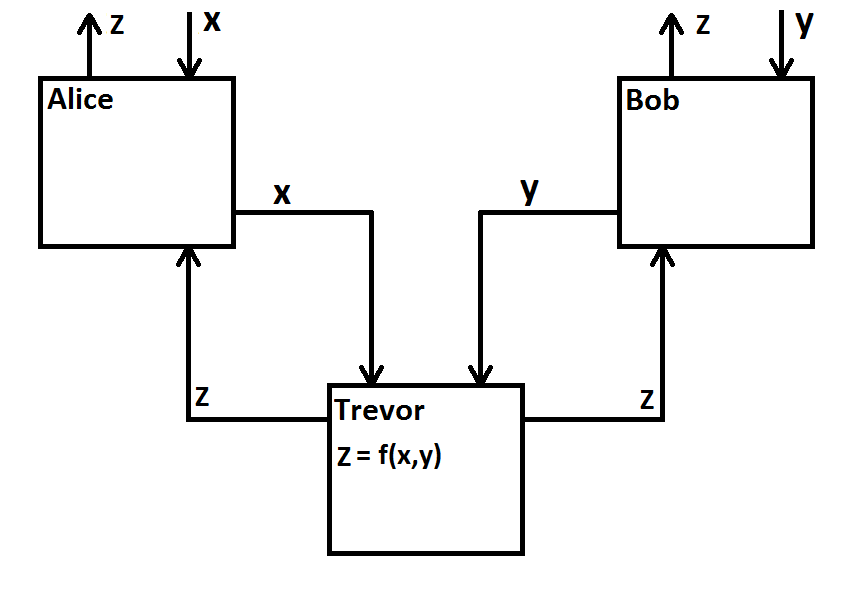
\includegraphics[scale=0.6]{Images/IdealModel}
		% Diagram. One big one will do me thinks.
	\end{frame}


	\begin{frame}
		\frametitle{Security Definitions}
		
		\begin{itemize}

		\item We measure the security of an SMC protocol in terms of what adversaries it is secure against, we define adversaries in terms of their capabilities.

		\item We say that an SMC protocl is secure against an adversary if the adversary can achieve no more than they would be able to achieve attacking the Ideal Model.

		\item We focus on three adversaries,
			\begin{itemize}
			\item Semi-Honest 
			\item Malicious 
			\item Covert
			\end{itemize}
		\end{itemize}
		% Acknowledge we're skipping over Static and Active corruption issues.
	\end{frame}
	
	\begin{frame}
		\frametitle{Semi-Honest Adversaries}
		\begin{itemize}
			\item Semi-Honest(SH) adversaries are the weakest adversary we shall consider.
			\item They are sometimes also called ``honest, but curious''.
			\item SH adversaries are limited to looking at information given to them in the process of the protocol.
			\item They have to follow the protocol (they cannot cheat). 
			\item SH adversaries are very similar to traditional ``Passive'' adversaries.
		\end{itemize}
	\end{frame}

	\begin{frame}
		\frametitle{Malicious and Coverts Adversaries}
		\begin{itemize}
			\item Malicious adversaries are the strongest adversary.
			\item Malicious adversaries can use any arbitrary strategy. We do not assume that they follow the protocol.
			\item Further more Malicious Adversaries are willing for their cheating to be noticed.
			\bigskip
			\item Covert Adversaries slightly weaker than Malicious Adversaries.
			\item Covert Adversaries can also use any arbitrary strategy, but they are adverse to being caught.
			\item They are willing to accept a certain probability of getting caught.
		\end{itemize}
	\end{frame}

	\begin{frame}
		\frametitle{Oblivious Transfer}
		\begin{itemize}
			\item A key component we will need later is Oblivious transfer(OT).
			\item Security definitions for OTs is are very similar to SMC, though we don't really look at the Covert case.
      
			\begin{figure}[!htb]
				\centering
				\begin{columns}
					\begin{column}{0.45\textwidth}
						\centering
						\textbf{Receiver}\\
						Inputs : $b \in \{0, 1\}$\\
						Outputs : $X_b$\\
					\end{column}

					\begin{column}{0.45\textwidth}
						\centering
						\textbf{Sender}\\
						Inputs : $X_1$, $X_2$\\
						Outputs : $\emptyset$\\
					\end{column}
				\end{columns}
				\caption{ Definition of the functionality of a one-out-of-two OT protocol. Note k-out-of-n OT is also possible.\label{fig:OTformalDef}}
			\end{figure}
		\end{itemize}
	\end{frame}


	\begin{frame}
		\frametitle{Even-Goldreich-Lempel Semi Honest OT}
		\begin{figure}[!htb]
			\begin{tabular}[!htb]{p{6cm} p{6cm}}
				\textbf{Receiver} & \textbf{Sender}\\
				Inputs : $b \in \{0, 1\}$ & Inputs : $X_0$, $X_1$\\
				Outputs : $X_b$ & Outputs : $\emptyset$\\
			\end{tabular}

			\begin{itemize}
				\setlength{\itemsep}{0.5pt}
				\setlength{\parskip}{0pt}
				\setlength{\parsep}{0pt}

 				\item \textbf{Receiver:} Generates a public/private key pair $(E, D)$, where E is the public key.\\
				\item \textbf{Receiver:} Sets $PK_b = E$, choose $PK_{1-b}$ at random from the same distribution as the public keys. Send $PK_0$ and $PK_1$ to the Sender.\\
				\item \textbf{Sender:} Encrypt $X_0$ using $PK_0$ as $C_0$ and encrypt $X_1$ using $PK_1$ as $C_1$. Send $C_0$ and $C_1$ to the Receiver.\\
				\item \textbf{Receiver:} Receives $C_0$ and $C_1$, then decrypt $C_b$ using $D$. Output this decrypted value.
			\end{itemize}

			\caption{The abstracted Even-Goldreich-Lempel protocol. Who can suggest why this is only Semi Honest? \label{fig:EvenGoldreichLempel}}
		\end{figure}
	\end{frame}

	\begin{frame}
		\frametitle{Yao Garbled Circuits}
		\begin{itemize}
			\item The basic concept of Yao Garbled Circuits is that one party constructs a binary circuit corresponding to the function to be computed.
			\item For wire $w_i$ we denote the value of the wire as $b_i$, we generate two random ``garble value'', denote these by $k_i^0$ and $k_i^1$.
			\item We then generate a random permutation for each wire $w_i$, denote this by $\pi_i$.
			\item For each gate we create an encryption table indexed by $c_i$ and $c_j$ (where the gates input wires are $w_i$ and $w_j$).
		\end{itemize}

	\end{frame}


	\begin{frame}
		\frametitle{Yao Garbled Circuits}

		\begin{columns}
			\begin{column}{0.4\textwidth}
				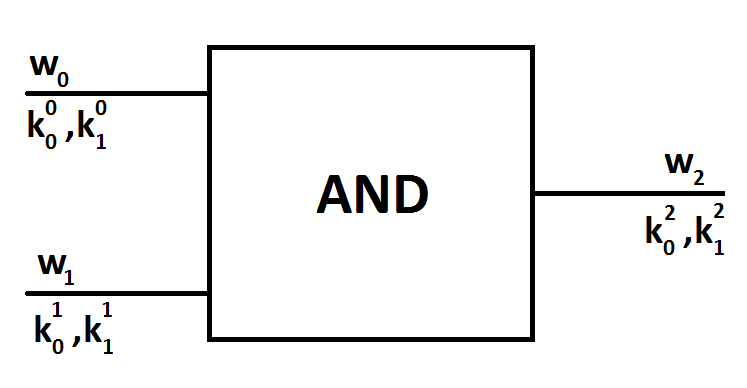
\includegraphics[scale=0.3]{Images/BasicGarbling}
			\end{column}

			\begin{column}{0.55\textwidth}
				\begin{tabular}[!htb]{c | c || c}
					$b_0$ & $b_1$ & \\
					\hline
					\hline
					$0$ & $0$ & $E_{k_0^0}(E_{k_1^0}(k_2^0 \Vert b_2))$\\
					\hline
					$0$ & $1$ & $E_{k_0^0}(E_{k_1^1}(k_2^0 \Vert b_2))$\\
					\hline
					$1$ & $0$ & $E_{k_0^1}(E_{k_1^0}(k_2^0 \Vert b_2))$\\
					\hline
					$1$ & $1$ & $E_{k_0^1}(E_{k_1^1}(k_2^1 \Vert ))$\\
				\end{tabular}
			\end{column}
		\end{columns}

	\end{frame}

	\begin{frame}
		\frametitle{Yao Garbled Circuits}
		\centering
		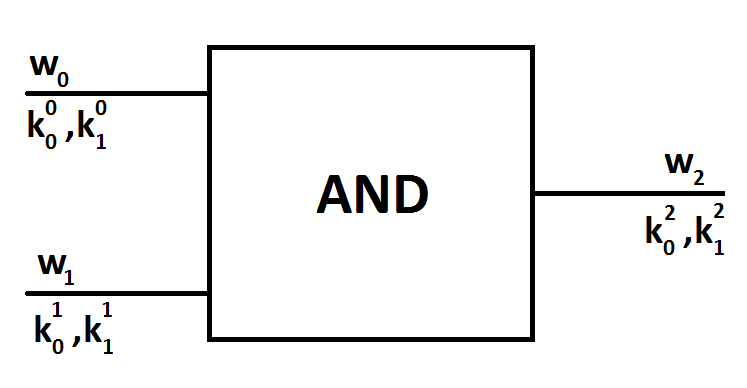
\includegraphics[scale=0.4]{Images/BasicGarbling}

		$$c_0, c_1 : E_{k_0^{b_0}}(E_{k_1^{b_1}}(k_2^{G(b_0, b_1)} \Vert c_2))$$
		where $c_i = \pi_i(b_i)$ and $G(., .)$ is the function taking the input of the gate and returning the output of the gate.
	\end{frame}

	\begin{frame}
		\frametitle{Yao Garbled Circuits}
		\begin{itemize}
			\item We extend this to all gates of the circuit.
			\item The Builder then sends the circuit to the Executor, stripped of the values of the permutations and keys.
			% Note this means we're basically sending the 
			\item The Builder then sends the keys relating to its inputs for its input wires.
			\item The Builder also sends the permutations for the Executors input wires and the Executors output wires.
		\end{itemize}

	\end{frame}


\end{document}













